%% ---------------------------------------------------------------------
%% 04 - KẾT QUẢ VÀ THẢO LUẬN
%% ---------------------------------------------------------------------

\section{Kết quả và thảo luận}\label{sec:results}

Mục này trình bày kết quả thực nghiệm của thuật toán Funnel Tree kết hợp Thủ tục 2
(\emph{Clip off Funnels}) được cài đặt bằng Python, đối sánh với chương trình
tham chiếu trên 5 mesh nhỏ và phân tích trường hợp điển hình trên lưới địa hình
vách dốc. Trọng tâm gồm: (1) đánh giá tổng thể trên 9 mesh kiểm thử; (2) phân
tích chuyên sâu lưới \texttt{cliff} kèm trực quan hóa; (3) mô tả cơ chế cắt tỉa
trong cài đặt hiện tại; (4) phân tích sai số và thảo luận ý nghĩa ứng dụng.

\subsection{Kết quả thực nghiệm tổng thể trên các lưới đa diện}

Thuật toán được thực thi trên 9 mesh \texttt{.off} của bộ dữ liệu. Kết quả được đối soát theo ba tiêu chí:
\begin{description}
  \item[Độ sai lệch so với chương trình tham chiếu]
    ($|L_{\text{Funnel}}-L_{\text{ref}}|/L_{\text{ref}}$): so sánh độ dài polyline
    đến từng đỉnh với đường tham chiếu độc lập; reference được làm tròn 4 chữ số
    thập phân.
  \item[Khả năng chạy và tính nhất quán nội tại] với 4 mesh không có reference,
    kiểm tra route được dựng cho mọi đỉnh đích và độ dài polyline dựng lại khớp
    độ dài nội tại mà phép lan truyền tính được.
  \item[Quy mô tìm kiếm] ghi nhận số lần lan truyền và việc bật/tắt cắt tỉa trong
    route JSON, thay cho số nút cây và số sự kiện clip mà phiên bản cũ ghi riêng.
\end{description}
Bảng~\ref{tab:ket-qua-tong-the} tổng hợp các chỉ số thu được.

\begin{table*}[!t]
  \caption{Kết quả chạy Funnel Tree trên 9 lưới đa diện. $P$ là số lần lan truyền;
    sai số tương đối chỉ tính cho 5 mesh có file tham chiếu. Dấu ``---'' nghĩa là
    không có reference độc lập.}
  \label{tab:ket-qua-tong-the}
  {\fontsize{7}{8.6}\selectfont
  \begin{adjustbox}{max width=\textwidth}
  \begin{tabular}{@{}lrrrrrrl@{}}
    \toprule
    \textbf{Lưới đa diện} & $V$ & $F$ & \textbf{Nguồn $s$} & $P$
      & \textbf{Sai số tương đối lớn nhất} & \textbf{Trung bình} & \textbf{Reference} \\
    \midrule
    \texttt{cliff}       &  7 & 10  & 1 &  3 & $1{,}7\times10^{-5}$ & $2{,}6\times10^{-6}$ & Có \\
    \texttt{cube}        &  8 & 12  & 0 &  1 & --- & --- & Không \\
    \texttt{J17}         & 10 & 16  & 1 &  1 & $4{,}8\times10^{-6}$ & $1{,}7\times10^{-6}$ & Có \\
    \texttt{L}           & 12 & 20  & 1 &  3 & $9{,}0\times10^{-10}$ & $7{,}5\times10^{-11}$ & Có \\
    \texttt{icosahedron} & 12 & 20  & 0 &  1 & --- & --- & Không \\
    \texttt{star}        & 16 & 28  & 0 &  9 & $6{,}7\times10^{-6}$ & $8{,}3\times10^{-7}$ & Có \\
    \texttt{dome}        & 25 & 40  & 0 &  1 & --- & --- & Không \\
    \texttt{demo\_mesh}  & 31 & 62  & 1 & 20 & $3{,}6\times10^{-7}$ & $8{,}5\times10^{-8}$ & Có \\
    \texttt{terrain}     & 49 & 72  & 0 & 26 & --- & --- & Không \\
    \bottomrule
  \end{tabular}
  \end{adjustbox}}
  \par\smallskip
  {\footnotesize $P$ lấy từ \texttt{stats.propagations} của route JSON; sai số
  tương đối lấy từ kết quả đối chiếu. Mọi lần chạy đều bật cắt tỉa.}
\end{table*}

Nhận xét tổng quan:
\begin{itemize}
  \item Trên 5/5 lưới có dữ liệu đối chiếu chuẩn (\texttt{cliff}, \texttt{J17},
    \texttt{L}, \texttt{star}, \texttt{demo\_mesh}), tổng cộng 76 đỉnh được so,
    không có failure ở ngưỡng tương đối $10^{-4}$. Sai số tương đối lớn nhất là
    $1{,}7\times10^{-5}$ (\texttt{cliff}), phát sinh từ việc reference chỉ giữ
    bốn chữ số thập phân; các mesh còn lại có sai số nhỏ hơn một bậc.
  \item Bốn mesh không có reference (\texttt{cube}, \texttt{icosahedron},
    \texttt{dome}, \texttt{terrain}) vẫn dựng được route cho mọi đỉnh đích, với
    $P=1$, $1$, $1$ và $26$. Đây là kiểm tra khả năng chạy trên bề mặt lồi, bề mặt
    mở và bề mặt có lỗ, không phải đối chiếu độ dài với một bộ giải thứ hai.
  \item Mọi route JSON ghi \texttt{clipping=true}; cài đặt hiện tại không phát
    sinh log từng sự kiện clip, nên bài báo không báo số lần cắt cụt cụ thể. Cơ
    chế cắt tỉa được mô tả định tính ở Mục~\ref{sec:clip}.
\end{itemize}

\begin{code}[!t]
  \lstinputlisting[style=jsoncode]{Code/compare_excerpt.json}
  \caption{Trích kết quả đối chiếu của \texttt{cliff}: thông tin mesh,
    nguồn, dung sai, sai số tương đối và danh sách độ dài từng đỉnh. Trường
    \texttt{paths} là nguồn của Bảng~\ref{tab:ket-qua-tong-the} và
    Bảng~\ref{tab:cliff-output}.}
  \label{code:compare}
\end{code}

\subsection{Nghiên cứu trường hợp điển hình: địa hình vách dốc}

Để làm rõ cơ chế vận hành từ khâu đọc dữ liệu hình học, dựng cây đến truy hồi
polyline, nghiên cứu phân tích chi tiết lưới \texttt{cliff} ($V=7$, $F=10$,
$E=15$). Đây là mô hình tiêu biểu cho địa hình đô thị hiểm trở với các sườn nghiêng
và vách đá dốc đứng.

\subsubsection{Mô hình bài toán và dữ liệu đầu vào}

Bài toán đặt trong bối cảnh: trạm chỉ huy và tiếp vận UAV đặt tại chân vách đá
$s=1$ tọa độ $(0,0,0)$. UAV cần vận chuyển hàng cứu trợ khẩn cấp lên điểm cao nhất
tại đỉnh vách đá $v=6$ tọa độ $(0,2,3)$, đồng thời thiết lập các tuyến đường tối ưu
đến toàn bộ các mốc quan trắc trung gian $v\in\{0,2,3,4,5\}$.

Dữ liệu đầu vào chuẩn \texttt{cliff.off} được biểu diễn như sau:
\begin{itemize}
  \item Dòng tiêu đề xác định kích thước hình học: $V=7$ đỉnh, $F=10$ mặt tam giác,
    $E=15$ cạnh.
  \item Tọa độ 7 đỉnh trong không gian $\R^3$: $v_0(2;2;0)$, $v_1(0;0;0)$ (nguồn
    $s$), $v_2(3;-2;0)$, $v_3(2;-1;3)$, $v_4(1;-0{,}5;1{,}5)$,
    $v_5(0{,}91865;1{,}45943;1{,}5)$ và $v_6(0;2;3)$ (đỉnh vách).
  \item Danh sách 10 mặt tam giác được định nghĩa bởi bộ ba chỉ số đỉnh:
    $f_0(0,1,5)$, $f_1(1,4,5)$, $f_2(3,5,6)$, $f_3(3,4,6)$, $f_4(4,5,6)$,
    $f_5(1,2,4)$, $f_6(2,3,4)$, $f_7(2,0,5)$, $f_8(2,3,5)$ và $f_9(1,0,2)$.
\end{itemize}

\subsubsection{Trực quan hóa không gian ba chiều}

Hình~\ref{fig:cliff-visual} minh họa kết quả không gian 3D do
công cụ trực quan hóa kết xuất, thể hiện cấu trúc lưới tam giác và các
đường tham chiếu tỏa ra từ đỉnh nguồn $s=1$.

\begin{figure}[!t]
  \centering
  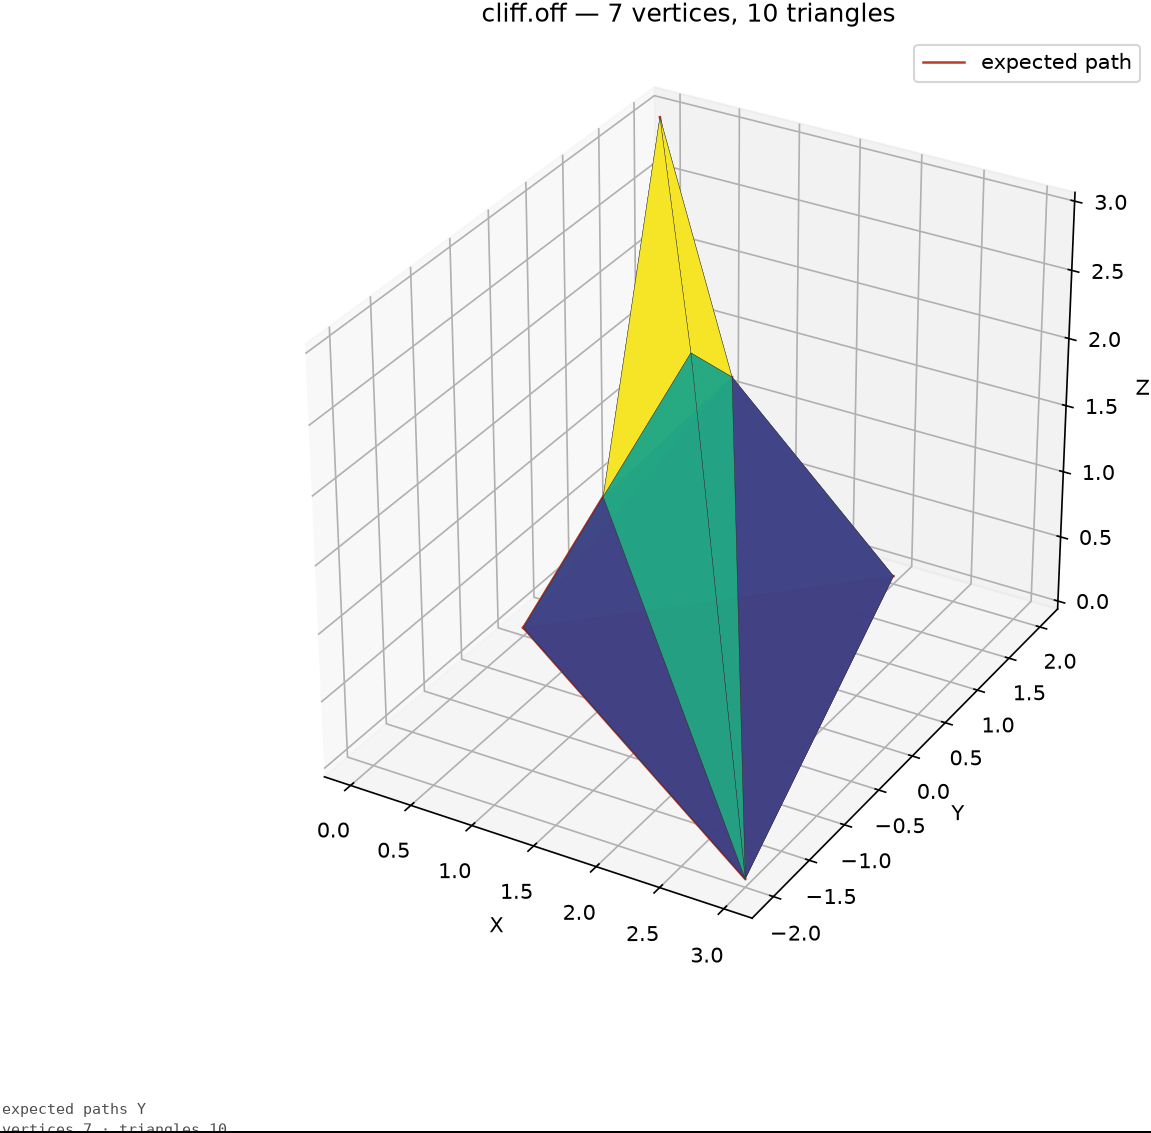
\includegraphics[width=0.95\linewidth]{Figures/crop/repo_cliff.png}
  \caption{Trực quan hóa đường tham chiếu trên bề mặt địa hình \texttt{cliff}
    với đỉnh nguồn $s=1$, kết xuất bởi công cụ trực quan hóa. Các đường màu đỏ là
    polyline tham chiếu; độ dài do
    Funnel Tree tính được đối chiếu ở Bảng~\ref{tab:cliff-output}.}
  \label{fig:cliff-visual}
\end{figure}

Từ Hình~\ref{fig:cliff-visual}, hai đặc trưng hình học quan trọng được làm sáng tỏ:
\begin{enumerate}
  \item Các polyline tham chiếu được vẽ trên cùng một mesh; độ dài do Funnel Tree trả về được đối chiếu với
    chúng ở Bảng~\ref{tab:cliff-output}. Ảnh không chồng hai lớp đường, nên việc
    so khớp được thực hiện bằng số liệu chứ không bằng mắt.
  \item Tuyến đường từ trạm $s=1$ lên đỉnh cao nhất $v=6$ cắt ngang qua cạnh
    $[4,5]$ tại điểm nội tại $(0,9356;1,0513;1,5000)$ --- đây là ưu thế của Funnel
    Tree so với xấp xỉ qua đỉnh của đồ thị rời rạc.
\end{enumerate}

\subsubsection{Dữ liệu đầu ra và phân tích polyline}

Bảng~\ref{tab:cliff-output} phân tích chi tiết polyline kết quả cho lưới
\texttt{cliff}, đối chiếu giữa đường tham chiếu trong
đường tham chiếu và độ dài do Funnel Tree trả về trong kết quả đối chiếu.

\begin{table*}[!t]
  \caption{Chi tiết polyline đường đi ngắn nhất từ nguồn $s=1$ trên lưới
    \texttt{cliff}.}
  \label{tab:cliff-output}
  {\fontsize{7}{8.6}\selectfont
  \begin{tabular}{@{}rr>{\raggedright\arraybackslash}p{150pt}r>{\raggedright\arraybackslash}p{118pt}@{}}
    \toprule
    \textbf{Đích $v$} & \textbf{Số điểm $m$} & \textbf{Tọa độ các điểm trên
      polyline} & \textbf{Chiều dài} & \textbf{Đặc điểm hình học} \\
    \midrule
    $0$ & 2 & $[0;0;0]\to[2;2;0]$ & 2,8284 & Đoạn thẳng trên mặt phẳng đáy
      $\triangle 102$ \\
    $1$ & 2 & $[0;0;0]\to[0;0;0]$ & 0,0000 & Đỉnh nguồn $s=1$ (phân đoạn suy
      biến) \\
    $2$ & 2 & $[0;0;0]\to[3;-2;0]$ & 3,6056 & Đoạn thẳng trên mặt phẳng đáy
      $\triangle 102$ \\
    $3$ & 3 & $[0;0;0]\to[1;-0{,}5;1{,}5]\to[2;-1;3]$ & 3,7417 & Gãy góc qua đỉnh gờ
      trung gian $v=4$ \\
    $4$ & 2 & $[0;0;0]\to[1;-0{,}5;1{,}5]$ & 1,8708 & Đoạn thẳng trực tiếp trên mặt
      sườn $\triangle 124$ \\
    $5$ & 2 & $[0;0;0]\to[0{,}9186;1{,}4594;1{,}5]$ & 2,2855 & Đoạn thẳng trực tiếp
      trên mặt sườn $\triangle 105$ \\
    $6$ & 3 & $[0;0;0]\to[0{,}9356;1{,}0513;1{,}5]\to[0;2;3]$ & 4,0632 &
      \textbf{Cắt ngang cạnh $[4,5]$ tại điểm trắc địa nội tại} \\
    \bottomrule
  \end{tabular}}
\end{table*}

\subsection{Cơ chế cắt tỉa của Thủ tục 2}\label{sec:clip}

Điểm mấu chốt giúp thuật toán hướng tới độ phức tạp $O(n^2)$ là việc kiểm soát
sự bùng nổ số lượng phễu khi lan truyền qua các mặt kề nhau. Khi hai phễu xuất
phát từ các nhánh khác nhau cùng tiếp cận và chiếm một đỉnh $v$ qua cùng cạnh
$[p,q]$ (\emph{occupy vertex $v$}), Thủ tục 2 so sánh bộ đo độ dài và góc để cắt
nhánh kém tối ưu. Trong cài đặt hiện tại, cắt tỉa là một tùy chọn boolean của
\texttt{solve\_targets}; mọi route JSON và file đối chiếu đều ghi
\texttt{clipping=true}.

Cài đặt không phát sinh log cho từng sự kiện cắt tỉa, nên bài báo không báo số
lần clip hay số nút cây cụ thể. Thay vào đó, Bảng~\ref{tab:ket-qua-tong-the} ghi
số lần lan truyền $P$ của từng mesh: $P=3$ trên \texttt{cliff}, $1$ trên
\texttt{J17} và \texttt{cube}, $3$ trên \texttt{L}, $9$ trên \texttt{star}, $20$
trên \texttt{demo\_mesh}, $26$ trên \texttt{terrain}. Với 5 mesh có reference,
toàn bộ 76 đỉnh đều khớp độ dài trong ngưỡng $10^{-4}$ khi bật cắt tỉa. Đây là
bằng chứng cắt tỉa không làm sai kết quả trên bộ dữ liệu này, không phải chứng
minh chặn $O(n^2)$ cho mọi đầu vào.

\subsection{Phân tích sai số và tính ổn định số học}

Vấn đề then chốt trong tính toán hình học 3D là sự tích lũy sai số dấu phẩy động
(\emph{floating-point rounding errors}) khi chuỗi các hàm lượng giác
$\cos,\sin,\arccos,\arcsin$ được gọi liên tiếp qua nhiều tầng mở rộng. Nghiên cứu
đã kiểm định sai số số học và ghi nhận các kết quả sau:
\begin{description}
  \item[Kẹp giá trị (\emph{value clamping})] Đối số của \texttt{math.acos} được
    kẹp trong $[-1,1]$ trước khi gọi, triệt tiêu lỗi miền xác định
    (\emph{domain error}) do sai số tính toán làm tỉ số vượt quá $1+10^{-16}$.
  \item[Độ ổn định qua nhiều mặt] Trên lưới phức tạp nhất \texttt{demo\_mesh}
    ($F=62$), sai số tương đối lớn nhất so với reference là
    $3{,}6\times10^{-7}$ và trung bình $8{,}5\times10^{-8}$, cùng bậc với các
    mesh nhỏ hơn. Trên \texttt{cliff}, nơi có đường cắt ngang cạnh, sai số tương
    đối lớn nhất là $1{,}7\times10^{-5}$ và vẫn nằm dưới ngưỡng $10^{-4}$.
  \item[Giới hạn diễn giải] Các sai số trên là sai số độ dài so với reference làm
    tròn bốn chữ số, không phải chứng minh ổn định số học cho mọi cấu hình; repo
    không kèm bộ test nhiễu hay kiểm tra độ dài trên mặt phẳng.
\end{description}

\subsection{Thảo luận và ý nghĩa ứng dụng cho bài toán đàn UAV}

\subsubsection{So sánh ưu thế với nhánh phương pháp Chen và Han}

Theo đối sánh trong bài báo gốc \cite{an2024funnel}, Funnel Tree tránh bước trải
phẳng toàn cục (\emph{planar unfolding}) của nhánh thuật toán truyền thống và mang
lại ba ưu thế:
\begin{enumerate}
  \item Nhờ biên trái của phễu luôn là đường trắc địa thẳng nhất (\emph{straightest
    geodesic}), toàn bộ các tính toán mở rộng chỉ cần áp dụng định luật cos và sin
    cục bộ, loại bỏ chi phí duy trì ma trận biến đổi đẳng cự.
  \item Mỗi nút phễu chỉ lưu một số hằng hữu hạn, giảm đáng kể chi phí bộ nhớ so
    với cửa sổ (\emph{windows}) trên từng cạnh.
  \item Cài đặt hoàn chỉnh chỉ phụ thuộc NumPy và thư viện chuẩn Python, không
    cần thư viện hình học, mà vẫn đạt độ chính xác tương đương chương trình tham
    chiếu.
\end{enumerate}

\subsubsection{Ý nghĩa thực tiễn đối với hệ thống UAV bầy đàn đô thị}

Kết quả thực nghiệm trên các lưới địa hình mở ra hướng ứng dụng trực tiếp:
\begin{description}
  \item[Dẫn đường bám sát bề mặt (\emph{terrain-following navigation})] Trong môi
    trường đô thị có mật độ nhà cao tầng dày đặc hoặc vùng cấm bay tầm cao, quỹ
    đạo bay bám theo bề mặt đa diện của các công trình (mái nhà, sườn tháp) giúp
    UAV ẩn mình dưới tầm quét radar và tận dụng luồng gió nâng địa hình để tiết
    kiệm năng lượng.
  \item[Tối ưu hóa đa điểm giao hàng] Funnel Tree là thuật toán một nguồn -- mọi
    đích. Chỉ với một lần dựng cây từ kho hàng $s$, toàn bộ lộ trình tối ưu tới
    mọi khách hàng đều được xác định đồng thời, không cần chạy lại thuật toán cho
    từng UAV riêng lẻ.
  \item[Nền tảng cho bài toán đàn robot không va chạm] Tập hợp các polyline trắc
    địa cung cấp khung lộ trình không gian chính xác, làm tiền đề để áp dụng các
    thuật toán điều phối thời gian (\emph{Time-Space Reservation}) nhằm tránh xung
    đột giữa các UAV trong đàn ở pha nghiên cứu tiếp theo.
\end{description}

\subsection{Hướng phát triển}

Dựa trên những kết quả đạt được, các định hướng công việc tiếp theo gồm:
\begin{description}
  \item[Kết nối giao tiếp với UAV thực] Cài đặt giao thức truyền lộ trình trắc địa
    từ máy tính điều khiển tới bộ điều khiển bay của UAV, đồng thời thêm nhánh xử
    lý tín hiệu phản hồi vị trí để hiệu chỉnh quỹ đạo theo thời gian thực.
  \item[Mô phỏng trên bản đồ chi tiết] Chuyển đổi bản đồ thành phố chi tiết thành
    lưới tam giác hóa để mô phỏng tuyến bay trong môi trường đô thị, kế thừa mô
    hình \texttt{city.glb}. Phần này đã được triển khai bước đầu ở
    Mục~\ref{sec:gazebo}.
  \item[Tối ưu thuật toán trên mesh lớn] Đánh giá và cải tiến hiệu năng cài đặt
    Python khi làm việc với mesh có mật độ mặt lớn hơn (hàng trăm nghìn tam giác),
    hướng tới khả năng dựng funnel tree trong thời gian chấp nhận được cho bài
    toán dẫn đường đô thị quy mô rộng.
\end{description}
